
% Author: PokMan Ho pok.ho19@imperial.ac.uk
% Script: LogisticTmp.tex
% Desc: `LaTex` report framework -- Logistic Growth
% Input: none
% Output: none
% Arguments: 0
% Date: Oct 2019

\documentclass[a4paper, 11pt]{article}
\usepackage[margin=1in]{geometry}
\usepackage{hyperref}

%% test insert graphs
\usepackage{graphicx}
\graphicspath{ {../results/} } %% <https://www.overleaf.com/learn/latex/Inserting_Images>

%% test insert variables
\newcommand{\text}{hihihi} %% <https://stackoverflow.com/questions/1211888/is-there-any-way-i-can-define-a-variable-in-latex>

\title{Still testing}
\author{PokMan Ho (CID: 01786076)}
\date{}

%% citation
\usepackage[%
autocite    = superscript,
backend     = bibtex,
sortcites   = true,
style       = nature,
]{biblatex}
\bibliography{../reference/LogRef.bib} %% <https://tex.stackexchange.com/questions/6805/bib-library-file-in-a-different-directory-how-to-use-mendeley-centralised-b>

\begin{document}
	\maketitle
	hihi\autocite{zwietering1994modeling}
	\section*{Abstract}
	\section*{Introduction}
	\section*{Methods}
	\section*{Results}
	\begin{figure}[h]
		\centering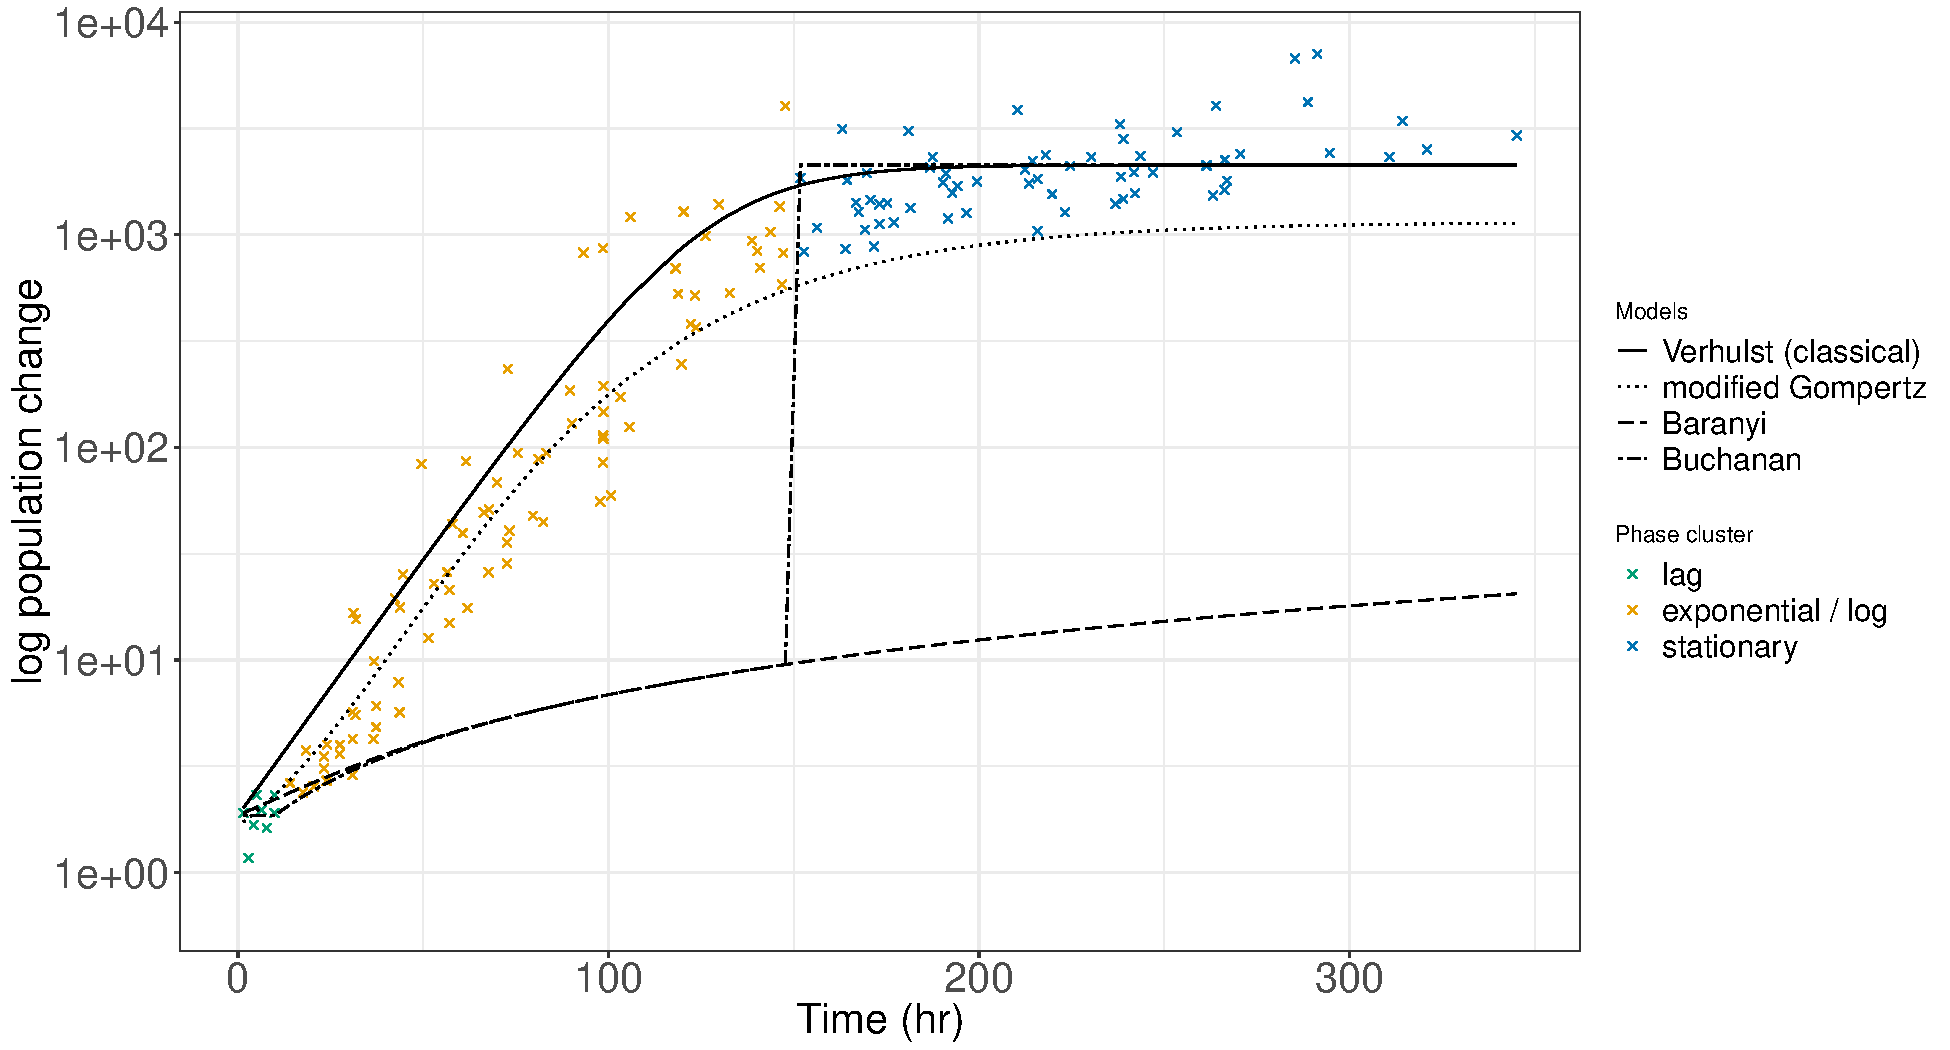
\includegraphics[width=10cm]{Log_data.pdf}
	\end{figure}
	\section*{Discussion}
	\section*{Conclusion}
	\section*{References}
	\nocite{*}\printbibliography
\end{document}